% !TeX root = ../skript.tex
% !TeX spellcheck = de_DE

\section{Visualisierung}
Das oben erwähnte Gleichungssystem haben wir im Javascript-Code verwendet, um die Resultate des Lorenzsystems auszurechnen. Der folgende Code beschreibt das oben vorgestellte Lorenz-Modell in JavaScript. Nachfolgend ist eine Aufstellung aller Variablen im Code und in den Formeln oberhalb.

% TODO: Beschreibung warum Durchlauf Unterschied macht, da Rückkopplungen unaufgelöst, und welche Probleme es nicht löst.
\begin{figure}
	\begin{lstlisting}[style=C]
x = arr[i].x + ((sigma * y) - (sigma * x)) * delta;
y = arr[i].y + ((-x * z) + (rho * x) - y) * delta;
z = arr[i].z + ((x * y) - (beta * z)) * delta;
		\end{lstlisting}
\end{figure}

\begin{table}[]
	\begin{tabular}{| c | c | c | c |}
		\hline
		\textbf{Bedeutung} & \textbf{Mathematisches Symbol} & \textbf{Variable im Code} & \textbf{Anfangswert}\\\hline
		Zeitschritt & $ \Delta $ & \texttt{delta} & 0.1 \\\hline
		Rayleigh Zahl & $ \sigma $ & \texttt{sigma} & 10 \\\hline
		Prandtl Zahl & $\varrho $ & \texttt{rho} & 28 \\\hline
		Wärmeausdehnung & $\beta $ & \texttt{beta}  & $ \frac{8}{3} $ \\\hline
	\end{tabular}
	\caption{Code variablen und ihre Werte\label{CodeVariablen}}
\end{table}

Die $ x, y $ Variablen in der 1. Gleichung ist noch mit dem Wert des vorherigen Durchgangs besetzt und deshalb eine Annäherung um den echten Wert. Das Gleiche gilt für alle Werte, die vor der Ausführung noch nicht gesetzt sind. 
Beim ersten Durchgang wird 0.1 als Startwert angenommen um zu verhindern, dass das Gleichungssystem gelöst ist. 

Wenn $ \vec{0} $ eingesetzt wird löst sich das Gleichungssystem auf $ \vec{0} $. Da das Ergebnis in der nächsten Runde wieder eingesetzt wird, wird das Gleichungssystem über alle Runden $ \vec{0} $ ausgeben. Um dieses Verhalten zu verhindern, lassen wir den Algorithmus etwas neben $ \vec{0} $ starten, nämlich bei $ \vec{0.1} $.

\begin{figure}
	\begin{lstlisting}[style=C, language=C++]
calculate(rho = 28, sigma = 10, beta = 8 / 3) {
	const it = 2500;
	
	let x = 0.1;
	let y = 0.1;
	let z = 0.1;
	const delta = 0.01;
	
	const pos = [];
	pos.push(new THREE.Vector3(x, y, z));
	
	for (let i = 0; i < it; i += 1) {
		x = pos[i].x + ((sigma * y) - (sigma * x)) * delta;
		y = pos[i].y + ((-x * z) + (rho * x) - y) * delta;
		z = pos[i].z + ((x * y) - (beta * z)) * delta;
		pos.push(new THREE.Vector3(x, y, z));
	}
	
	return pos;
}
		\end{lstlisting}
		\caption{Algorithmus für Lorenz-Modell\label{AlgorithmusLorenz}}
\end{figure}


Der Algorithmus \ref{AlgorithmusLorenz} startet mit der Initialisierung der Variablen in \ref{CodeVariablen}. Auf Linie 10 wird der Startwert auch in den Ortsvektoren-Array \textit{pos} gespeichert. Damit können wir eine generelle Schleife programmieren, die sich nicht um den Spezialfall $ length(pos) = 0 $ kümmern muss.
Die Schleife wird 2500 mal durchlaufen. In welcher die Schleife die Werte des Lorenz-Modells in einem Array als 3D-Vektoren abgespeichert. Diese Ortsvektoren stellen die Position der Punkte im drei dimensionalen Raum dar.

Die Darstellungsobjekte an diesen Positionen besitzen die Form von \textit{Spheren}. Wir haben diese Form gewählt, da sie in 3D einem Punkt im XY-Koordinatensystem nachempfunden ist. Ein solches Objekt stellt einen Wert der Lorenzgleichungen dar.

Die Darstellung wird mittels \textit{WebGL}\cite{WebGL} im Browser gerendert. Da \textit{WebGL} eine komplexe 3D-Graphik-API von \textit{OpenGL} ist, haben wir auf dieser Technologie aufbauende Middleware \textit{WhitestormJS}\cite{whitestormJS} verwendet. Diese Middleware bietet uns eine vereinfachte Abstraktion, denn wir benötigen nur sehr wenige Standardfunktionen von \textit{WebGL}.

Für die Interaktiviät der Webpage mit Animationen bei den Seitenwechsel, Textboxen und Strukturierung des Codes ist die neue JavaScript Bibliothek \textit{VueJS}\cite{VueJS} zum Einsatz gekommen.

Dank diesen Helfern konnten wir innerhalb von etwa 30h Arbeit eine vollständige Simulationsumgebung für das Lorenz-Modell 68 mit folgenden Charakteristiken programmieren:

\begin{itemize}
	\item 3D-Visualisierung
	\item Drehen und Zoomen
	\item Sofortiges update von 3D Visualisierung bei Paramteränderung
	\item fixe 3D-Bilder deren Parameter durch den Betrachter unveränderbar sind
	\item Erklärungstext
\end{itemize}

\begin{figure}
	\centering	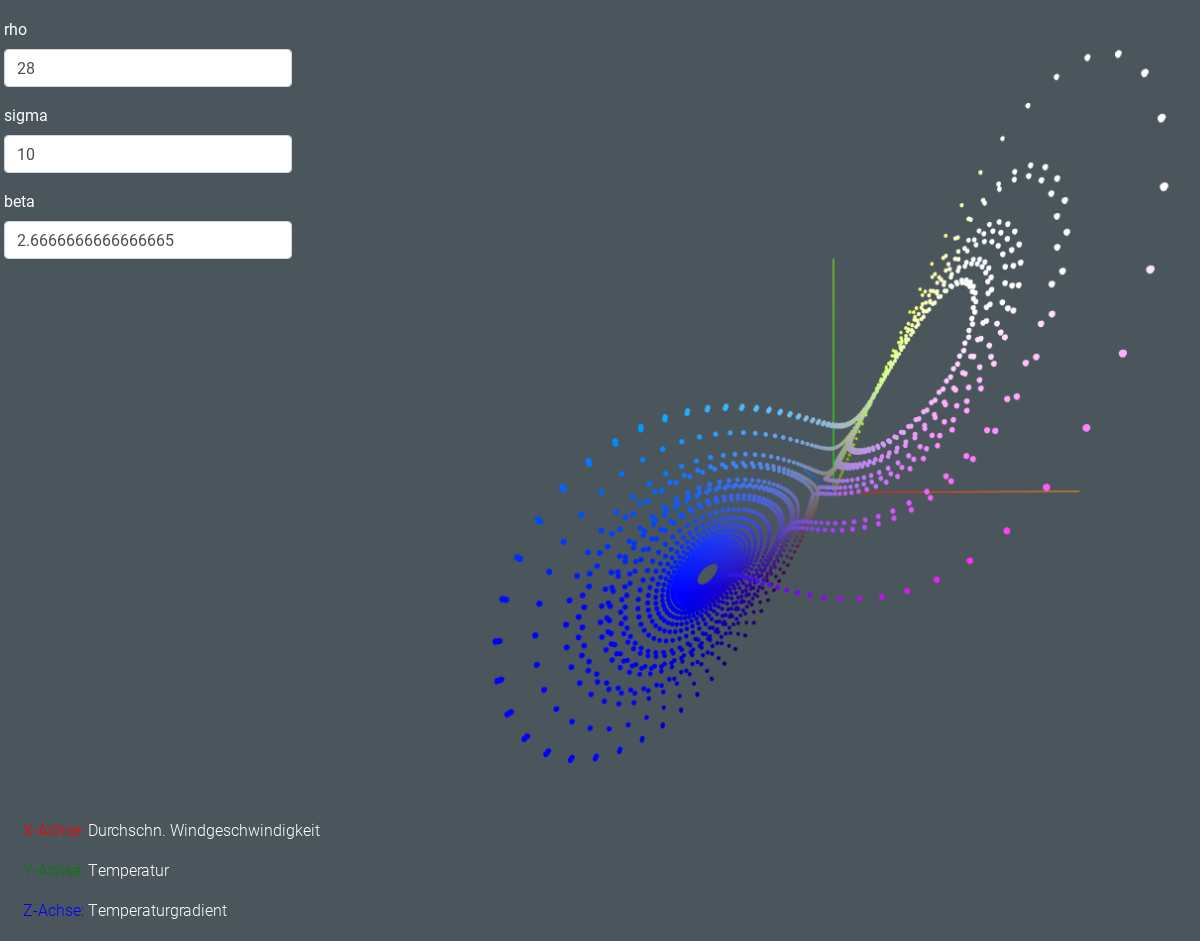
\includegraphics[height=7cm]{lorenz/assets/implementation/Visualisierung}
	\caption{Visualisierung Lorenz-Attraktor}
	\label{fig:visualisierung}
\end{figure}
